\documentclass[submit]{harvardml}

\course{CS181-S20}
\assignment{Assignment \#1}
\duedate{11:59pm February 7, 2020} 

\usepackage[OT1]{fontenc}
\usepackage[colorlinks,citecolor=blue,urlcolor=blue]{hyperref}
\usepackage[pdftex]{graphicx}
\usepackage{graphicx}
\graphicspath{ {./hw1/} }
\usepackage{caption}
\usepackage{subcaption}
\usepackage{fullpage}
\usepackage{soul}
\usepackage{amsmath}
\usepackage{amssymb}
\usepackage{color}
\usepackage{todonotes}
\usepackage{listings}
\usepackage{common}

\usepackage[mmddyyyy,hhmmss]{datetime}

\definecolor{verbgray}{gray}{0.9}

\lstnewenvironment{csv}{
  \lstset{backgroundcolor=\color{verbgray},
  frame=single,
  framerule=0pt,
  basicstyle=\ttfamily,
  columns=fullflexible}}{}
 

\begin{document}
\begin{center}
{\Large Homework 1: Linear Regression}\\
\end{center}

\subsection*{Introduction}
This homework is on different forms of linear regression and focuses
on loss functions, optimizers, and regularization. Linear regression 
will be one of the few models that we see that has an analytical solution.
These problems focus on deriving these solutions and exploring their 
properties. 

If you find that you are having trouble with the first couple
problems, we recommend going over the fundamentals of linear algebra
and matrix calculus (see links on website).  The relevant parts of the
cs181-textbook notes are Sections 2.1 - 2.7.  We strongly recommend reading the textbook before beginning the homework.

We also encourage you to first read the Bishop
textbook, particularly: Section 2.3 (Properties of Gaussian
Distributions), Section 3.1 (Linear Basis Regression), and Section 3.3
(Bayesian Linear Regression). (Note that our notation is slightly different but
the underlying mathematics remains the same!).

Please type your solutions after the corresponding problems using this
\LaTeX\ template, and start each problem on a new page.

Homeworks will be submitted through Gradescope. You will be added to the course Gradescope once you join the course Canvas page. If you haven?t received an invitation, contact the course staff through Piazza.

Please submit the \textbf{writeup PDF to the Gradescope assignment `HW1'}. Remember to assign pages for each question. 

Please submit your \textbf{\LaTeX file and code files to the Gradescope assignment `HW1 - Supplemental'}. 

You can use a \textbf{maximum of 2 late days} on this assignment.  Late days will be counted based on the latest of the two submissions.
\\
\newpage

%%%%%%%%%%%%%%%%%%%%%%%%%%%%%%%%%%%%%%%%%%%%%
% Problem 1
%%%%%%%%%%%%%%%%%%%%%%%%%%%%%%%%%%%%%%%%%%%%%
Problem 1: [Optimizing a Kernel, 15pts]

Kernel-based regression techniques are similar to nearest-neighbor
regressors: rather than fit a parametric model, they predict values
for new data points by interpolating values from existing points in
the training set.  In this problem, we will consider a kernel-based
regressor of the form:
\begin{equation*}
  f(x^*) = \frac{ \sum_{n} K(x_n,x^*) y_n  }{ \sum_{n} K(x_n,x^*) } 
\end{equation*}
where $(x_n,y_n)$ are the training data points, and $K(x,x')$ is a
kernel function that defines the similarity between two inputs $x$ and
$x'$. Assume that each $x_i$ is represented as a row vector, i.e. a
1 by $D$ vector where $D$ is the number of features for each data point. A popular choice of 
kernel is a function that decays as the distance between the two points increases, such as
\begin{equation*}
  K(x,x') = \exp(-||x-x'||^2_2) = \exp(-(x-x') (x-x')^T ) 
\end{equation*} 
However, the squared Euclidean distance $||x-x'||^2_2$ may not always
be the right choice.  In this problem, we will consider optimizing
over squared Mahalanobis distances
\begin{equation*}
  K(x,x') = \exp(-(x-x') W (x-x')^T ) 
  \label{eqn:distance}
\end{equation*} 
where $W$ is a symmetric $D$ by $D$ matrix.  Intuitively, introducing
the weight matrix $W$ allows for different dimensions to matter
differently when defining similarity.

\begin{enumerate}

\item Let $\{(x_n,y_n)\}_{n=1}^N$ be our training data set.  Suppose
  we are interested in minimizing the residual sum of squares.  Write down this
  loss over the training data $\mcL(W)$ as a function of $W$.
  
  Hint:  For each point $(x_i, y_i)$ in the training dataset, consider for which subset of training data you should sum kernel function $K$ over for each $f(x_i)$.
  
  \textbf{Answer:} 
  \begin{equation}
  \begin{split}
        L(W) &= \sum_{n} (y_n - \hat{y} )^2 \\
        &= \sum_{n} (y_n - f(x^*) )^2 \\
        &= \sum_{n} (y_n - \frac{ \sum_{n} K(x_n,x^*) y_n  }{ \sum_{n} K(x_n,x^*) } )^2\\
        &= \sum_{n} (y_n - \frac{ \sum_{n} \exp(-(x-x') W (x-x')^T ) y_n  }{ \sum_{n} \exp(-(x-x') W (x-x')^T ) } )^2
  \end{split}
  \end{equation}
  
  This works for most values. However, we will run into problems when the input $x$ values are the same. So, we need to add in a guardrail to make sure they're not the same point.
  
  \begin{equation}
      L(W)= \sum_{n} (y_n - \frac{ \sum_{j\neq i} \exp(-(x_j-x_i) W (x_j-x_i)^T ) y_n  }{ \sum_{j\neq i} \exp(-(x_j-x_i) W (x_j-x_i)^T ) } )^2
  \end{equation}

\item In the following, let us assume that $D = 2$.  That means that
  $W$ has three parameters: $W_{11}$, $W_{22}$, and $W_{12} = W_{21}$.
  Expand the formula for the loss function to be a function of these
  three parameters.

\textbf{Answer:}
Let $z = x_j-x_i$ 

such that 
\begin{equation}
\begin{split}
    K(x,x') &=\exp(-(x-x') W (x-x')^T \\
    &= \exp(-zWz^T)\\
    &= \exp(-\left[ {\begin{array}{cc}
   z_1 & z_2 \\
  \end{array} } \right] 
  \left[ {\begin{array}{cc}
   W_{11} & W_{12} \\
   W_{21} & W_{22} \\
  \end{array} } \right]
  \left[ {\begin{array}{1}
   z_1 \\
   z_2 \\
  \end{array} } \right]) \\
  &= \exp(- \left[ {\begin{array}{cc}
   z_1W_{11} + z_2W_{12} & z_1W_{21} + z_2W_{22} \\
  \end{array} } \right]
  \left[ {\begin{array}{1}
   z_1 \\
   z_2 \\
  \end{array} } \right]) \\
  &= \exp(-((z_1W_{11} + z_2W_{12})z_1 + (z_1W_{21} + z_2W_{22})z_2))\\
   &= \exp(-(z_1^2W_{11} + 2z_1z_2W_{12} + z_2^2W_{22}))\\
   &= \exp(-z_1^2W_{11} - 2z_1z_2W_{12} - z_2^2W_{22})
\end{split}
\end{equation}

Then, we can write the loss function as:

\begin{equation}
    L(W) = \sum_{n} (y_n - \frac{ \sum_{n} \exp(-z_1^2W_{11} - 2z_1z_2W_{12} - z_2^2W_{22}) y_n  }{ \sum_{n} \exp(-z_1^2W_{11} - 2z_1z_2W_{12} - z_2^2W_{22}) } )^2
\end{equation}

\item Consider the following data set:
\begin{csv}
x1 , x2 , y 
  0 , 0 , 0
  0 , .5 , 0
  0 , 1 , 0 
  .5 , 0 , .5
  .5 , .5 , .5
  .5 , 1 , .5
  1 , 0 , 1
  1 , .5 , 1
  1 , 1 , 1 
\end{csv}
And the following kernels:
\begin{equation*} 
W_1 = \alpha \begin{bmatrix}
  1 & 0 \\
  0 & 1 
\end{bmatrix}
\qquad
W_2 = \alpha \begin{bmatrix}
  0.1 & 0 \\
  0 & 1 
\end{bmatrix}
\qquad
W_3 = \alpha \begin{bmatrix}
  1 & 0 \\
  0 & 0.1 
\end{bmatrix}
\end{equation*} 
with $\alpha = 10$. Write some Python code to compute the loss with respect
to each kernel for the dataset provided above. Which kernel does best?  Why?  How does the choice of $\alpha$ affect the loss?  

\textbf{Answer:} $W_3$ performs the best, with a loss of $.025$. This is probably because $W_3$ weights $x_1$ more than $x_2$ such that $x_1$ matters more (i.e., is more predictive) than $x_2$. The choice of alpha affects the loss by determining the weighting of each interpolation point; as alpha approaches zero the surrounding points approach equal affect on the prediction and the bigger alpha gets, the more important the closest point becomes in predicting. 

\item Derive the gradients with respect to each of the parameters in
  $W$.
  
\textbf{Answer:}
\begin{equation}
  \begin{split}
        \nabla L(W) &= \begin{bmatrix}\frac{\partial}{\partial W_{11}}\sum_{n} (y_n - \hat{y} )^2 \\
        \frac{\partial}{\partial W_{12}}\sum_{n} (y_n - \hat{y} )^2  \\
        \frac{\partial}{\partial W_{22}}\sum_{n} (y_n - \hat{y} )^2 \end{bmatrix}\\
        &= \begin{bmatrix}- 2 \frac{\partial f}{\partial W_{11}}\sum_{n} (y_n - f(x) )\\
        - 2 \frac{\partial f}{\partial W_{12}}\sum_{n} (y_n - f(x) )\\
        - 2 \frac{\partial f}{\partial W_{22}}\sum_{n} (y_n - f(x) )\end{bmatrix}\\
        &= \begin{bmatrix}-2 \frac {\frac{\partial}{\partial W_{11}}[\sum_{n} K(x_n, x')y_n]\cdot \sum_n K (x_n,x') - \sum_{n} K (x_n, x')y_n \cdot \frac{\partial}{\partial W_{11}} [\sum_{n} K (x_n, x')]}{(\sum_{n} K (x_n, x'))^2}\sum_{n} (y_n - f(x) )\\
        -2 \frac {\frac{\partial}{\partial W_{12}}[\sum_{n} K(x_n, x')y_n]\cdot \sum_n K (x_n,x') - \sum_{n} K (x_n, x')y_n \cdot \frac{\partial}{\partial W_{12}} [\sum_{n} K (x_n, x')]}{(\sum_{n} K (x_n, x'))^2}\sum_{n} (y_n - f(x) )\\
        -2 \frac {\frac{\partial}{\partial W_{22}}[\sum_{n} K(x_n, x')y_n]\cdot \sum_n K (x_n,x') - \sum_{n} K (x_n, x')y_n \cdot \frac{\partial}{\partial W_{22}} [\sum_{n} K (x_n, x')]}{(\sum_{n} K (x_n, x'))^2}\sum_{n} (y_n - f(x) )\end{bmatrix}\\
        &= \begin{bmatrix}-2 \frac {\sum_{n} \frac{\partial K}{\partial W_{11}} (x_n, x')y_n \cdot \sum_n K (x_n,x') - \sum_{n} K (x_n, x')y_n \cdot \sum_{n} \frac{\partial K}{\partial W_{11}} (x_n, x')}{(\sum_{n} K (x_n, x'))^2}\sum_{n} (y_n - f(x) \\
        -2 \frac {\sum_{n} \frac{\partial K}{\partial W_{12}} (x_n, x')y_n \cdot \sum_n K (x_n,x') - \sum_{n} K (x_n, x')y_n \cdot \sum_{n} \frac{\partial K}{\partial W_{12}} (x_n, x')}{(\sum_{n} K (x_n, x'))^2}\sum_{n} (y_n - f(x))\\
        -2 \frac {\sum_{n} \frac{\partial K}{\partial W_{22}} (x_n, x')y_n \cdot \sum_n K (x_n,x') - \sum_{n} K (x_n, x')y_n \cdot \sum_{n} \frac{\partial K}{\partial W_{22}} (x_n, x')}{(\sum_{n} K (x_n, x'))^2}\sum_{n} (y_n - f(x)
        \end{bmatrix}\\
        &= \begin{bmatrix}-2 \frac {\sum_{n} K (x_n, x')y_n(-z_1^2) \cdot \sum_n K (x_n,x') - \sum_{n} K (x_n, x')y_n \cdot \sum_{n} K (x_n, x')(-z_1^2)}{(\sum_{n} K (x_n, x'))^2}\sum_{n} (y_n - f(x) )\\
        -2 \frac {\sum_{n} K (x_n, x')y_n(-z_1z_2) \cdot \sum_n K (x_n,x') - \sum_{n} K (x_n, x')y_n \cdot \sum_{n} K (x_n, x')(-z_1z_2)}{(\sum_{n} K (x_n, x'))^2}\sum_{n} (y_n - f(x) )\\
        -2 \frac {\sum_{n} K (x_n, x')y_n(-z_2^2) \cdot \sum_n K (x_n,x') - \sum_{n} K (x_n, x')y_n \cdot \sum_{n} K (x_n, x')(-z_2^2)}{(\sum_{n} K (x_n, x'))^2}\sum_{n} (y_n - f(x) )\end{bmatrix}\\
  \end{split}
  \end{equation}

\item Bonus:  Code up a gradient descent to
  optimize the kernel for the data set above.  Start your gradient
  descent from $W_1$.  Report on what you find.\\
  Gradient descent is discussed in Section 3.4 of the cs181-textbook notes and Section 5.2.4 of Bishop, and will be covered later in the course! 

\end{enumerate}



\newpage

%%%%%%%%%%%%%%%%%%%%%%%%%%%%%%%%%%%%%%%%%%%%%
% Problem 2
%%%%%%%%%%%%%%%%%%%%%%%%%%%%%%%%%%%%%%%%%%%%%

Problem 2: Kernels and kNN, 10pts

Now, let us compare the kernel-based approach to an approach based on
nearest-neighbors.  Recall that kNN uses a predictor of the form

  \begin{equation*}
    f(x^*) = \frac{1}{k} \sum_n y_n \mathbb{I}(x_n \texttt{ is one of k-closest to } x^*)
  \end{equation*}

 where $\mathbb{I}$ is an indicator variable. For this problem, you will use the same kernels as Problem 1, and dataset \verb|data/p2.csv|.

\begin{enumerate}

\item Make 6 plots using the kernel distance given by $W_1$ from Problem 1.  In each plot,
  you will plot the predicted value of $y$ as the color of each point (grayscale between $0$ and $1$) given $x_1$
  (horizontal axis) and $x_2$ (vertical axis).  For $x_1$ and $x_2$,
  use a grid spaced every 0.1 for $x_1=0$ to $x_1=1$ and $x_2=0$ to
  $x_2=1$.  
  
  For the first three plots, use the kernel-based predictor
  varying $\alpha = \{0.1,3,10\}$.  For the next three plots, use
  the kNN predictor with $\alpha = 1$, $k=\{1,5,15\}$.  Print the least squares loss for each of the 6 plots.
  
  You may choose to use some starter Python code to create your plots provided in \verb|T1_P2.py|.  Please \textbf{write your own implementation of kNN} for full credit.  Do not use external libraries to find nearest neighbors.

\textbf{Answer:} 

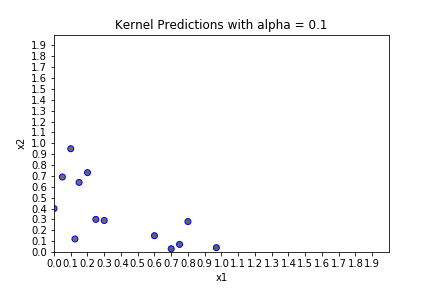
\includegraphics[scale=.5]{Kernel Predictions with alpha = 0.1.png}
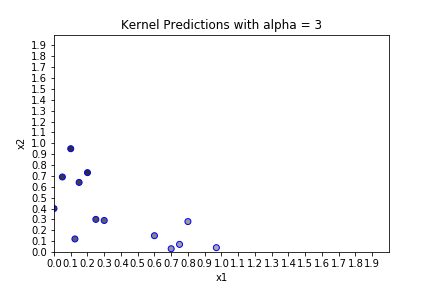
\includegraphics[scale=.5]{Kernel Predictions with alpha = 3.png}\\
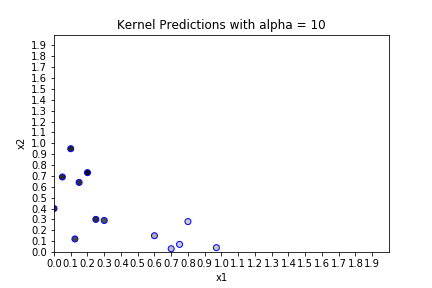
\includegraphics[scale=.5]{Kernel Predictions with alpha = 10.png}
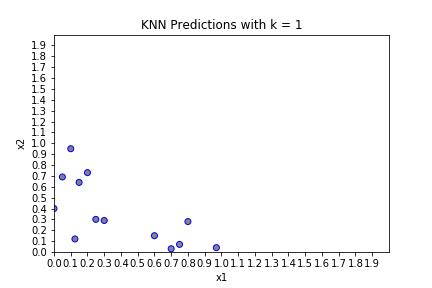
\includegraphics[scale=.5]{KNN Predictions with k = 1.png}\\
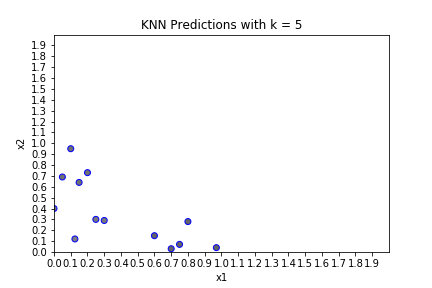
\includegraphics[scale=.5]{KNN Predictions with k = 5.png}
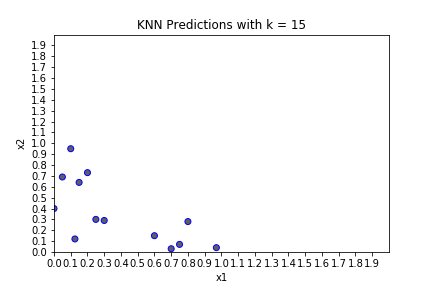
\includegraphics[scale=.5]{KNN Predictions with k = 15.png}\\
The Least Squares Loss for alpha = 0.1 is 1.840 \\
The Least Squares Loss for alpha = 3 is 0.620 \\
The Least Squares Loss for alpha = 10 is 0.390 \\
The Least Squares Loss for k = 1 is 0.839 \\
The Least Squares Loss for k = 5 is 0.469 \\
The Least Squares Loss for k = 15 is 1.923 \\


\item Do any of the kernel-based regression plots look like the 1NN?
  The 15NN?  Why or why not?\\

\textbf{Answer:} 
Yes, the kernel-based regression with $\alpha = 10$ looks like the 1KNN. This is because the $\alpha$ makes the weight of more distant points very small, which means the model relies heavily on the 1 closest point. The K=1 model similarly relies on the first closest point. \\
Additionally, $\alpha = .1$ looks similar to 15NN, because both models rely on all the points in the data, and the $\alpha$ makes it so that all of the points carry similar weight.\\

\item Do you think that there will always be a version of kernel
  regression (based on varying $\alpha$) that looks like a kNN for any
  $k$, for a fixed distance or kernel function?  Why or why not?\\

\textbf{Answer:} 
No, there is one example where this would not be true: a dataset with three points that are all equal distance, a KNN = 1 would randomly pick a point, while a kernel would get the average.\\

\item Why did we not vary $\alpha$ for the kNN approach?  \\ 

\textbf{Answer:} For kernel regression, changing the $\alpha$ changes the weights of the surrounding points in a model where all of the surrounding points are taken into account. However, for KNN we are picking points using a constant, so even though a change in $\alpha$ would change the distances of the surrounding points, we would still be choosing those closest K points to make a prediction and a change in $\alpha$ wouldn't change the neighbors that are used.

\end{enumerate}



\newpage 

%%%%%%%%%%%%%%%%%%%%%%%%%%%%%%%%%%%%%%%%%%%%%
% Problem 3
%%%%%%%%%%%%%%%%%%%%%%%%%%%%%%%%%%%%%%%%%%%%%

Problem 3: Deriving Linear Regression, 10pts

In class, we noted that the solution for the least squares linear regressions ``looked'' like a ratio of covariance and variance terms.  In this problem, we will derive that.  Let us assume the following generative process for our data:

\begin{eqnarray*}
  x &\sim N(0,\Sigma_x) \\
  \epsilon &\sim N(0,\sigma^2)\\
  y | x, \epsilon &= w^Tx + \epsilon 
  \end{eqnarray*}
  
Assume 1-dimensional $x$, $\epsilon$, and $y$, and that $x$ is independent of $\epsilon$.

\begin{enumerate}

\item Provide a formula for $\Sigma_{yx} = E_{x, y}[yx]$ based on the above generative model.

\textbf{Answer:}
\begin{equation}
  \begin{split}
    \Sigma_{yx} &= E_{x, y}[yx]\\
    &= E[E[yx|x \epsilon]] \\
    &= E[E[w^Tx] + E[x \epsilon]] \\
    &= E[w^TE[x^2]] \\
    &= w^T\Sigma_x
    \end{split}
\end{equation}


\item Provide a formula to estimate $E_{x, y}[yx]$ given observed data $\{(x_n,y_n)\}_{n=1}^N$.

\textbf{Answer:}
\begin{equation}
  \begin{split}
  E_{x, y}[yx] = \frac{1}{N}\sum_{n=1}(y_n x_n)
  \end{split}
\end{equation}

\item Moment terms like $E_{x, y}[yx]$, $E_{x, y}[xx^T]$, etc. can easily be
  estimated from the data (like you did above).  Write down an
  expression for the optimal $w^*$ which minimizes expected squared residual loss 
  in terms of moments
  (e.g. $\mu_x,\Sigma_x,\Sigma_{yx},\sigma$). Does your expression for optimal $w^*$ match the optimal $w^*$ for least squares linear regression derived in Section 2.6 of the cs181-textbook?
  
\testbf{Answer:}
\begin{equation}
    \begin{split}
        L(w^*) &= E_{x, \epsilon} [(y - \hat{y})^2] \\
        &= E_{x, \epsilon} [(y - \hat{w} x)^2] \\
        &= E_{x, \epsilon}[y^2 - 2y\hat{w}x - \hat{w}x^2]\\
        &= E_{x, \epsilon}[y^2] - E_{x, \epsilon}[2y\hat{w}x] -E_{x, \epsilon}[\hat{w}x^2]\\
        &= E_{x, \epsilon}[y^2] - \hat{w} E_{x, \epsilon}[2yx] -E_{x, \epsilon}[\hat{w}x^2]\\
        \frac{\partial}{\partial \hat{w}}&= E_{x, \epsilon}[y^2] - \hat{w} E_{x, \epsilon}[2yx] -E_{x, \epsilon}[\hat{w}x^2] \\
        &= 0 - E_{x, \epsilon}[2yx] - 2\hat{w} E_{x, \epsilon}[x^2]\\
        0 &= - E_{x, \epsilon}[2yx] - 2\hat{w} E_{x, \epsilon}[x^2]\\
        \frac{2E_{x,\epsilon}[yx]}{-2E_{x,\epsilon}[x^2]} &= \hat{w}\\
        \frac{\Sigma_{yx}}{\Sigma_{x}} &= \hat{w}\\
    \end{split}
\end{equation}

\item Now, suppose the data $x$ were generated from
  $N(\mu_x,\Sigma_x)$.  Write an expression for $w^*$ in terms of
  moments (as above).  
  
\testbf{Answer:}
\begin{equation}
    \begin{split}
        L(w^*) &= E_{x, \epsilon} [(y - \hat{y})^2] \\
        &= E_{x, \epsilon} [(y - \hat{w} x)^2] \\
        &= E_{x, \epsilon}[y^2 - 2y\hat{w}x - \hat{w}x^2]\\
        &= E_{x, \epsilon}[y^2] - E_{x, \epsilon}[2y\hat{w}x] -E_{x, \epsilon}[\hat{w}x^2]\\
        &= E_{x, \epsilon}[y^2] - \hat{w} E_{x, \epsilon}[2yx] -E_{x, \epsilon}[\hat{w}x^2]\\
        \frac{\partial}{\partial \hat{w}}&= E_{x, \epsilon}[y^2] - \hat{w} E_{x, \epsilon}[2yx] -E_{x, \epsilon}[\hat{w}x^2] \\
        &= 0 - E_{x, \epsilon}[2yx] - 2\hat{w} E_{x, \epsilon}[x^2]\\
        0 &= - E_{x, \epsilon}[2yx] - 2\hat{w} E_{x, \epsilon}[x^2]\\
        \frac{2E_{x,\epsilon}[yx]}{-2E_{x,\epsilon}[x^2]} &= \hat{w}\\
        \frac{\Sigma_{yx}}{\Sigma_{x}
        +\mu_x^2} &= \hat{w}\\
        \frac{\Sigma_{yx}}{\Sigma_{x}+0}
        &= \hat{w}\\
        \frac{\Sigma_{yx}}{\Sigma_{x}}
         &= \hat{w}\\
    \end{split}
\end{equation}

  
\item Would the formula for $w^*$ derived in (3.4) hold if the process generating the $x$'s
  were no longer Gaussian, but still had the same means, variances, and covariances?
  That is, $E[x]=\mu_x$, $Var[x]=\Sigma_x$, $Var[\epsilon] = \sigma^2$, and $E[yx] = \Sigma_{y x}$, but the distribution of $x$
  is not Gaussian?  

\testbf{Answer:} Yes, because we used the moments that are the same as the moments of the normal, but nothing we did in the 3.4 derivation was dependent on the features of the normal distribution.
  
\end{enumerate}

\\

\newpage
%%%%%%%%%%%%%%%%%%%%%%%%%%%%%%%%%%%%%%%%%%%%%
% Problem 4
%%%%%%%%%%%%%%%%%%%%%%%%%%%%%%%%%%%%%%%%%%%%%

Problem 4: Modeling Changes in Republicans and Sunspots, 15pts]
  
 The objective of this problem is to learn about linear regression
 with basis functions by modeling the number of Republicans in the
 Senate. The file \verb|data/year-sunspots-republicans.csv| contains the
 data you will use for this problem.  It has three columns.  The first
 one is an integer that indicates the year.  The second is the number
 of Sunspots observed in that year.  The third is the number of Republicans in the Senate for that year.
 The data file looks like this:
 \begin{csv}
Year,Sunspot_Count,Republican_Count
1960,112.3,36
1962,37.6,34
1964,10.2,32
1966,47.0,36
\end{csv}

You can see scatterplots of the data in the figures below.  The horizontal axis is the Year, and the vertical axis is the Number of Republicans and the Number of Sunspots, respectively.

\begin{center}
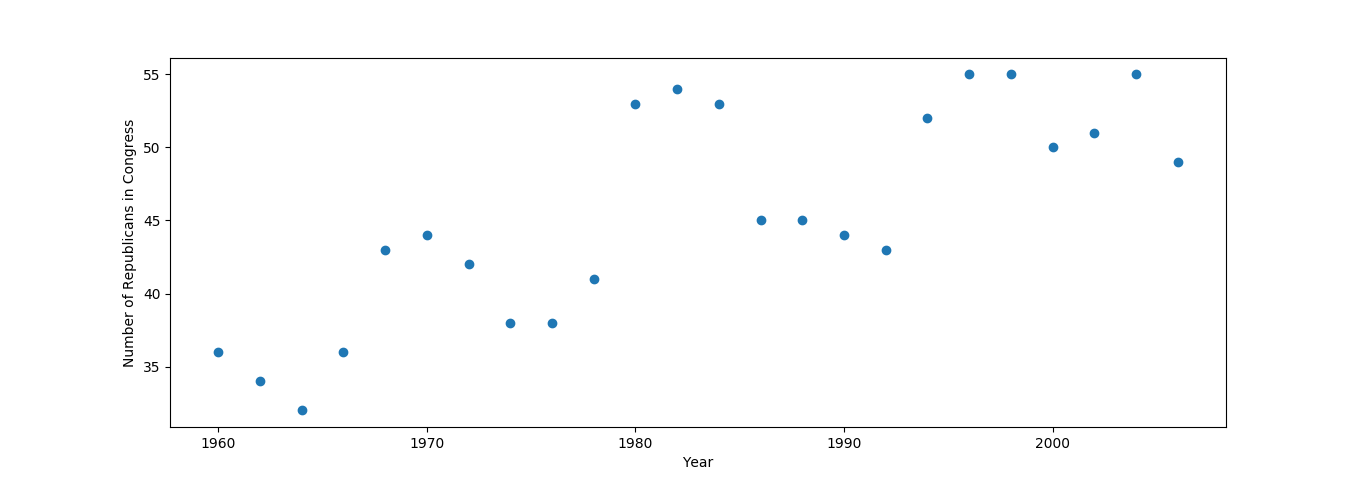
\includegraphics[width=.5\textwidth]{data/year-republicans}
\end{center}

\begin{center}
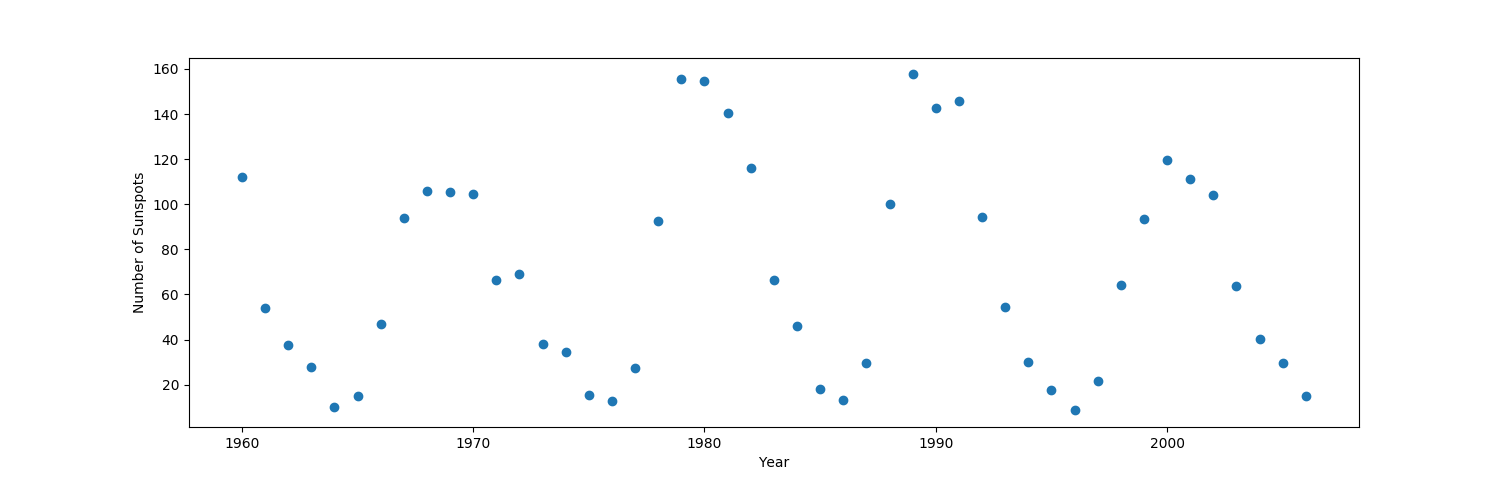
\includegraphics[width=.5\textwidth]{data/year-sunspots}
\end{center}

(Data Source: \url{http://www.realclimate.org/data/senators_sunspots.txt})\\
\vspace{-5mm}

\begin{enumerate}

\item In this problem you will implement ordinary least squares regression using 4 different basis functions for
\textbf{Year (x-axis)} v. \textbf{Number of Republicans in the Senate (y-axis)}. Some starter Python code
that implements simple linear regression is provided in \verb|T1_P3.py|.

First, plot the data and regression lines for each of the following sets of basis functions, and include
the generated plot as an image in your submission PDF. You will therefore make 4 total plots:

\begin{enumerate}
	\item[(a)] $\phi_j(x) = x^j$ for $j=1, \ldots, 5$\\
    ie, use basis $y = a_1 x^1 + a_2 x^2 + a_3 x^3 + a_4 x^4 + a_5 x^5$ for some constants $\{a_1, ..., a_5\}$. \\
    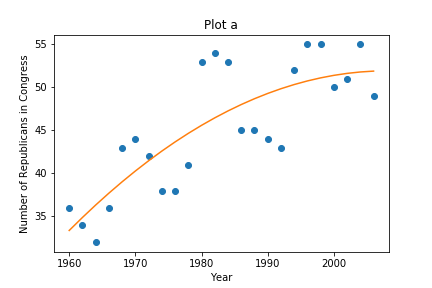
\includegraphics[width=.5\textwidth]{Plot a.png}\\
    The RSS = 424.878\\
    \item[(b)] $\phi_j(x) = \exp{\frac{-(x-\mu_j)^2}{25}}$ for $\mu_j=1960, 1965, 1970, 1975, \ldots 2010$ \\
    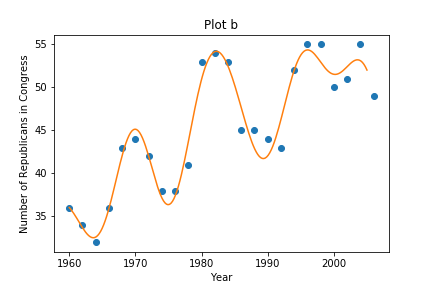
\includegraphics[width=.5\textwidth]{Plot b.png}\\
    The RSS = 54.273\\
	\item[(c)] $\phi_j(x) = \cos(x / j)$ for $j=1, \ldots, 5$ \\
	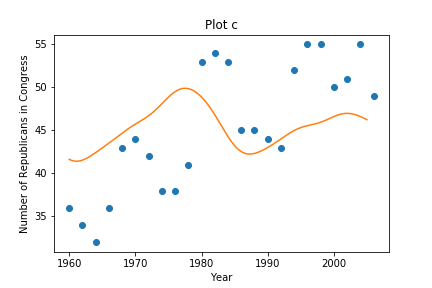
\includegraphics[width=.5\textwidth]{Plot c.png}\\
	The RSS = 1082.808\\
	\item[(d)] $\phi_j(x) = \cos(x / j)$ for $j=1, \ldots, 25$ \\
	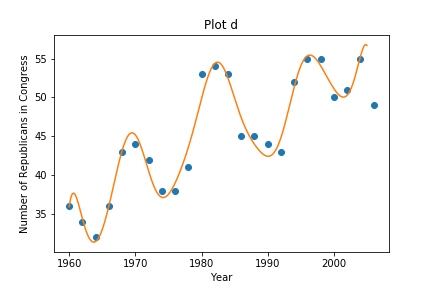
\includegraphics[width=.5\textwidth]{Plot d.png}\\
	The RSS = 38.8\\
\end{enumerate}
\vspace{-2mm}
{\footnotesize * Note: Be sure to add a bias term for each of the basis functions above.}

Second, for each plot include the residual sum of squares error.

\item Repeat the same exact process as above but for \textbf{Number of Sunspots (x-axis)} v. \textbf{Number of Republicans in the Senate (y-axis)}. Now, however, only use data from before 1985, and only use basis functions (a), (c), and (d) -- ignore basis (b). You will therefore make 3 total plots. For each plot make sure to also include the residual sum of squares error.

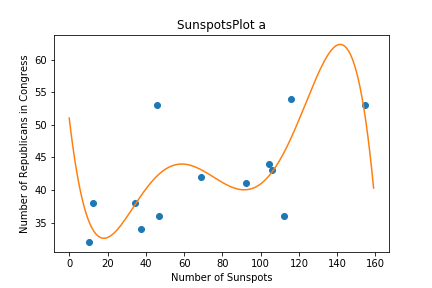
\includegraphics[width=.5\textwidth]{SunspotsPlot a.png}\\
The RSS = 351.228\\
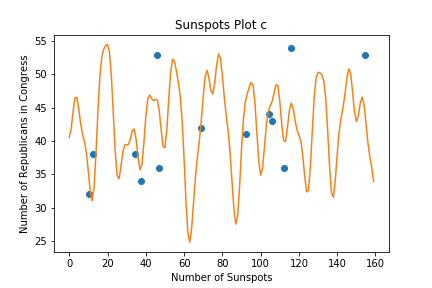
\includegraphics[width=.5\textwidth]{hw1/Sunspots Plot c.png}\\
The RSS = 375.107\\
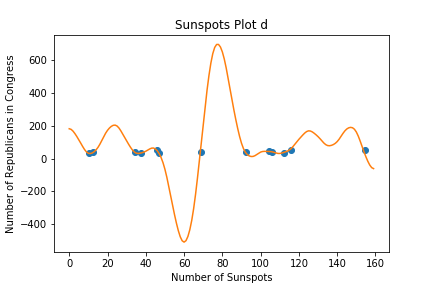
\includegraphics[width=.5\textwidth]{hw1/Sunspots Plot d.png}\\
The RSS = 5.906e-24\\

Which of the three bases (a, b, d) provided the "best" fit? \textbf{Choose one}, and keep in mind the generalizability of the model.\\ 

\textbf{Answer:} While basis function d has the smallest RSS (suggesting that it would be the best fit model), it seems to only perform well because it is over fit to the training data. This suggests that it wouldn't generalize and isn't a model that represents the true nature of the larger population. Because of this, I think that basis function a provides the best fit, because it doesn't seem over fit to the training data set and has a lower RSS than basis c.\\

Given the quality of this fit, do you believe that the number of sunspots controls the number of Republicans in the senate (Yes or No)?\\

\textbf{Answer:} Obviously, we can not claim a causal relationship between these two variables because we have no way to estimate counterfactuals and we did not perform random assignment (it would be impossible to do this). Additionally, the "best" basis (a) has a  high RSS, suggesting that there isn't a strong relationship. For these two reasons, I do not think number of sunspots controls the number of Republicans in the Senate. 
\end{enumerate}



\newpage
%%%%%%%%%%%%%%%%%%%%%%%%%%%%%%%%%%%%%%%%%%%%%
% Name and Calibration
%%%%%%%%%%%%%%%%%%%%%%%%%%%%%%%%%%%%%%%%%%%%%
\subsection*{Name}

\subsection*{Collaborators and Resources}
I got help from the TFs and other students in Office Hours. I also consulted the math book, Towards Data Science, and stack overflow.

\subsection*{Calibration}
Approximately how long did this homework take you to complete (in hours)? \\
Somewhere between 15-20 hours.

\end{document}



